\usetikzlibrary{arrows.meta}
\begin{frame}{size mismatch? (1)}
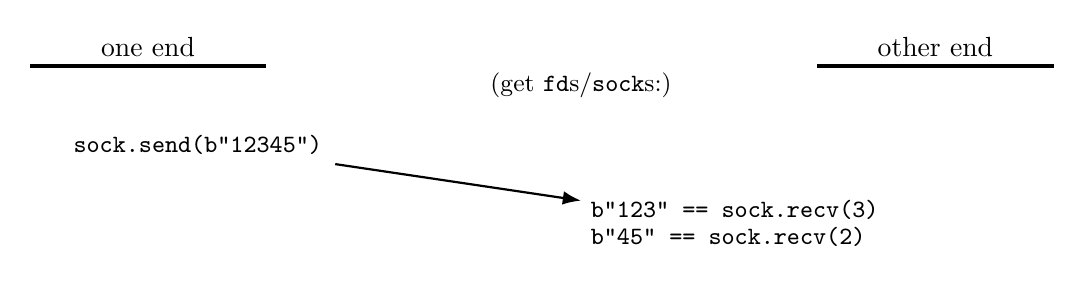
\begin{tikzpicture}
\tikzset{>=Latex}
\node[anchor=south] at (1.5, 0) {one end};
\draw[ultra thick] (0, 0) -- ++(3, 0);
\draw[ultra thick] (10, 0) -- ++(3, 0);
\node[anchor=south] at (11.5, 0) {other end};
\node[font=\small] at (7, -.25) {(get \texttt{fd}s/\texttt{sock}s:)};
\tikzset{
    function/.style={font=\fontsize{9}{10}\tt\selectfont,align=left},
}
\node[function,anchor=east] (write 1) at (4, -1) {
sock.send(b"12345")
};
\node[function,anchor=west] (read 1) at (7, -2) {
b"123" == sock.recv(3) \\
b"45" == sock.recv(2) 
};
\draw[thick,->] (write 1) -- (read 1);
\end{tikzpicture}
\end{frame}

\begin{frame}{size mismatch? (2)}
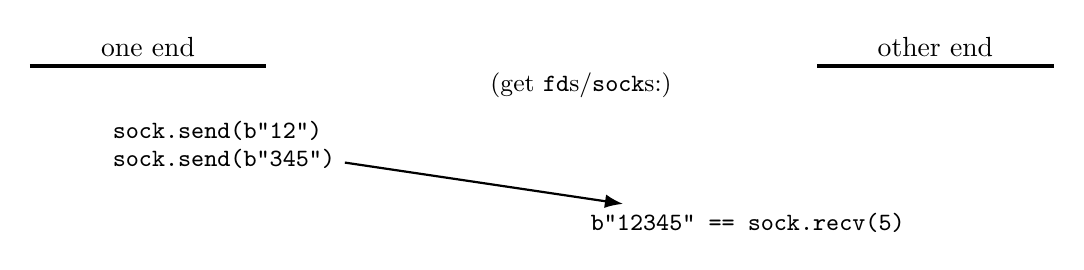
\begin{tikzpicture}
\tikzset{>=Latex}
\node[anchor=south] at (1.5, 0) {one end};
\draw[ultra thick] (0, 0) -- ++(3, 0);
\draw[ultra thick] (10, 0) -- ++(3, 0);
\node[anchor=south] at (11.5, 0) {other end};
\node[font=\small] at (7, -.25) {(get \texttt{fd}s/\texttt{sock}s:)};
\tikzset{
    function/.style={font=\fontsize{9}{10}\tt\selectfont,align=left},
}
\node[function,anchor=east] (write 1) at (4, -1) {
sock.send(b"12") \\
sock.send(b"345")
};
\node[function,anchor=west] (read 1) at (7, -2) {
b"12345" == sock.recv(5)
};
\draw[thick,->] (write 1) -- (read 1);
\end{tikzpicture}
\end{frame}

\begin{frame}{partial reads?}
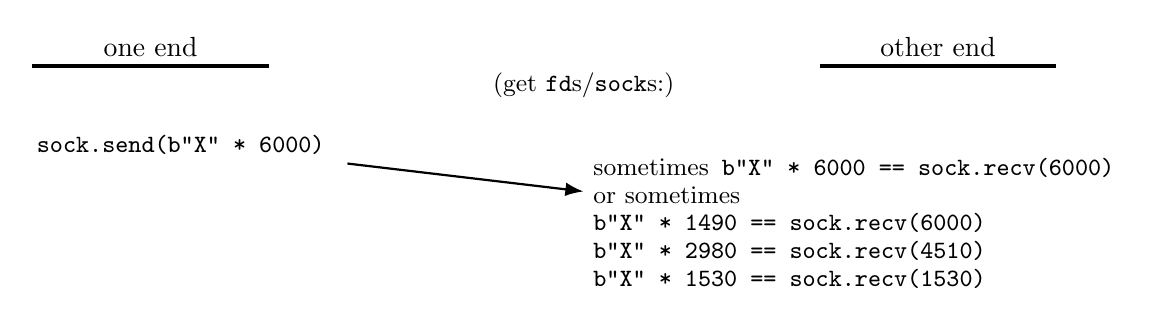
\begin{tikzpicture}
\tikzset{>=Latex}
\node[anchor=south] at (1.5, 0) {one end};
\draw[ultra thick] (0, 0) -- ++(3, 0);
\draw[ultra thick] (10, 0) -- ++(3, 0);
\node[anchor=south] at (11.5, 0) {other end};
\node[font=\small] at (7, -.25) {(get \texttt{fd}s/\texttt{sock}s:)};
\tikzset{
    function/.style={font=\fontsize{9}{10}\tt\selectfont,align=left},
}
\node[function,anchor=east] (write 1) at (4, -1) {
sock.send(b"X" * 6000)
};
\node[function,anchor=west] (read 1) at (7, -2) {
\textit{\normalfont sometimes} b"X" * 6000 == sock.recv(6000) \\
\textit{\normalfont or sometimes} \\
b"X" * 1490 == sock.recv(6000) \\
b"X" * 2980 == sock.recv(4510) \\
b"X" * 1530 == sock.recv(1530) 
};
\draw[thick,->] (write 1) -- (read 1);
\end{tikzpicture}
\end{frame}

\begin{frame}{partial writes}
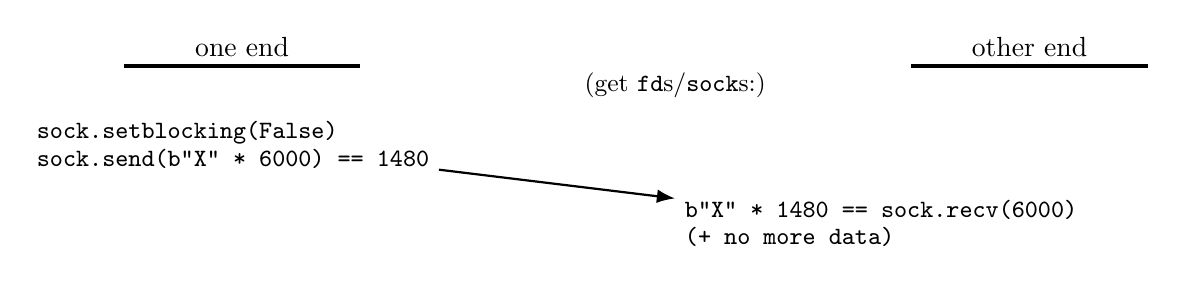
\begin{tikzpicture}
\tikzset{>=Latex}
\node[anchor=south] at (1.5, 0) {one end};
\draw[ultra thick] (0, 0) -- ++(3, 0);
\draw[ultra thick] (10, 0) -- ++(3, 0);
\node[anchor=south] at (11.5, 0) {other end};
\node[font=\small] at (7, -.25) {(get \texttt{fd}s/\texttt{sock}s:)};
\tikzset{
    function/.style={font=\fontsize{9}{10}\tt\selectfont,align=left},
}
\node[function,anchor=east] (write 1) at (4, -1) {
sock.setblocking(False) \\
sock.send(b"X" * 6000) == 1480
};
\node[function,anchor=west] (read 1) at (7, -2) {
b"X" * 1480 == sock.recv(6000) \\
(+ no more data)
};
\draw[thick,->] (write 1) -- (read 1);
\end{tikzpicture}
\end{frame}

\begin{frame}{partial reads/writes}
    \begin{itemize}
    \item read/recv can have read less than requested
        \begin{itemize}
        \item read of zero bytes = end of file
        \end{itemize}
    \item send/write can write less than requested\ldots \\
        but only on error or if non-blocking mode requested
    \end{itemize}
\end{frame}
